\chapter[SCP-099 肖像]{
    SCP-099 The Portrait\\
    SCP-099 肖像
}

\label{chap:SCP-099}

\begin{figure}[H]
    \centering
    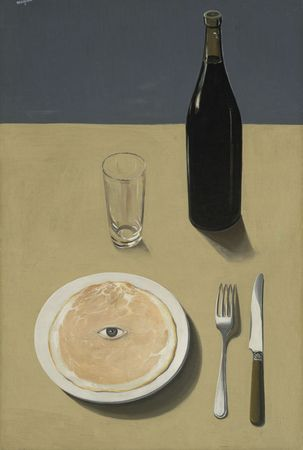
\includegraphics[width=0.5\linewidth]{images/SCP.099.jpg}
    \caption*{缺乏能造成心理伤害之必要细节的SCP-099小照片}
\end{figure}

\bb{项目编号:}SCP-099

\bb{项目等级:}Safe

\bb{特殊收容措施:}SCP-099应被保存于一个1M长75CM宽的固定于27号展览馆(Gallery 27)墙上的防火箱中,标准的气温和湿度调控应该被供给27号展览馆的该区域。因为该项目的内容,SCP-099只能在收容地点由等级2以上的人员观看,并只能在不小于5M的的距离上观察且一天的观察时间不能超过5分钟。当没有被观看时,收容099的箱子应该被电子锁密封。

\bb{描述:}SCP-099是一幅75CM长50CM宽,题为“肖像”(“The Portrait”)的画。是超现实主义画家雷内·马格利特(René Magritte)创作于1935年的作品。当这幅画的真品在小于5M以内的距离内被观察或是长时间被观察的时候,它将表现出能使人产生急性偏执狂以及长时间的慢性心理影响的模因效应,这幅画描画了一幅简单的静物画面,并且还有一只眼睛在画面上紧盯着观赏者。

一幅该画的复制品现在正在纽约现代艺术博物馆之中展出,该复制品之中的重要元素被移除以防有诱发急性偏执狂的可能。想要获得有关于改动的细节描述,请参阅文档099b。原作的精细复制品和照片仍然继承了SCP-099的模因性质。

那些在过近距离上观察SCP-099或是观察时间过久的人员将成为以下幻觉的受害者:任何的生物或是被描画出来的有着眼睛的生物都在死死地盯着他。在某些极端的情形之中,受害者报告说即便是没有生命的物体也都在对他进行着注视。

这些情况是如此地严重以至于受害者甚至会报告说它们能够感受到那些以后脑勺对着他们的个体的注视目光。取决于在原作之下曝光时离原作的距离,受害者有可能一生都被这种幻觉所折磨。最终将会发展成为严重的偏执症和惧群症(enochlophobia)。

\bb{附录:}SCP-099是从同为超现实主义画家凯伊·赛奇\footnote{\bb{译注:} Kay Sage}的私人收藏品之中被发现,最初的发现报告来自于机动特遣队Theta-6“粉色美洲豹”(Pink Panther)。塞奇夫人并没有注意到Theta-6的发现并且也没有发现SCP-099的掉包,虽然在收容之前的调查显示出她知晓SCP-099的性质并且对其免疫或是总是避免在过近的距离上观赏它。

马格利特在SCP-099在纽约现代艺术博物馆之中展出时仍然在世,之后他始终被置于基金会的监视之下直到他在1967年时去世,研究显示SCP-099的模因性质是有意为之的,虽然这种触发的力量和效果更像是无意的。基金会已经研究了马格利特的其他作品,但是其他的作品迄今为止没有表现出异常的模因性质。

\bb{武器化申请:}{[}数据删除]
